Polygonal boundary representations based on the concept of
halfedges \cite{k-ugpdd-99} are the fundamental of 
various mesh algorithms. A robust and efficient
design and implementation of such polyhedron data
structure is demanded by researchers and
developers. Based on the generic programming paradigm 
of the modern \CC\ design, the \emph{Computational 
Geometry Algorithms Library} (CGAL) provides a 
\emph{robust}, \emph{efficient} yet \emph{highly flexible} 
polyhedron data structure that aims to be the research
platform of the mesh algorithms. CGAL demonstrates
the possibility and powers of the generic geometry data structures
and algorithms. CGAL is standardized following the \CC\ STL 
and has emerged as the standard geometric computing library.

Being the platform for researching and developing
geometry algorithms, the CGAL polyhedron
data structure is 
\indent --- \emph{robust} for computational diffculties.
\indent --- \emph{efficient} on both aspects of speed and space.\\
\indent --- \emph{highly flexible} for specific mesh algorithms.\\
\noindent A complete set of the geometry entities and 
predications is also provided within CGAL. These reusable 
geometry components allows the design of complex algorithms 
within the same framework.
%No reinventing the wheel. The generic programming
%(and the object-oriented design) focuses on providing the
%reusable components, so we start with reusing the data structure.\\
The robustness, efficiency and flexibility of the CGAL polyhedron is
best evaluated through the implementation of several geometry algorithms.
Extensible algorithm models, based on CGAL, are expecting to speed up the
research and the development cycle, and therefore benefit the 
geometry processing community.

The intended audience of this paper are researchers, developers or
students in the graphics community developing algorithms around
polyhedron meshes. Experiences on the advanced \CC\ design, 
i.e.\ generic programming using templates, and knowledge 
of the halfedge data structure and related algorithms are 
prerequisites. The software design of the CGAL 
polyhedron is presented in section \ref{sect:}.
Implementations of different groups of geometry algorithms 
are then presented to furthermore evaluate the CGAL polyhedron.  
We first present a subdivision solution based on the 
generality of the CGAL polyhedron. The solution, decoupling 
the geometry rules from the refinement, grants users flexible 
controls of the geometry rules. Following the general
subdivision solution, a specific $\sqrt{3}$ subdivision 
is implemented to evaluate the performance of CGAL polyhedron. 
Remeshing techniques based on a combination of the 
CGAL polyhedron and Delaunay triangulation then demonstrate 
the versatility of the unified framework provided by CGAL.  
Last, several additional functionalities
such as minimum enclosing ball, convex hull, self intersection and
boolean operations are demonstrated on large meshes.  

%A mesh algorithm is usually implemented on a specific 
%designed data structure such as the quad-tree structure\cite{} 
%or patched mesh structure\cite{} for
%primal quadrisection subdivisions\cite{}.

%A graphics pipeline usually holds a geomotry 
%data structure for storage and rendering and other data structures for
%stages of specific geometry algorithms. The translations between stages
%invoke problems such as multiple storages, numeric
%inconsistency or performance deficiency. Most of the
%data structures are variations of the 
%edge-based mesh data structure. These variations are specialized 
%by replacing the entities types, which in geometry are the 
%position, the normal or other attributes such as color or 
%texture coordinates. 

%Most of the geometry algorithms combine two steps: \\
%\indent --- topology operations such as incidence traversal and refinement,\\
%\indent --- geometry operations such as position adjustment and 
%normal generation.\\ 
%\noindent A soft-coupled framework for geometry processing can then be built
%as a combination of three software components: the data structure, the
%topology operations and the geometry operations. With a flexible
%design based on the generic programming paradigm, researchers and
%developers can then focus on the key operations, i.e.\ geometry
%operations, of their algorithms.

%In this paper, we establish this soft-coupled framework of the
%geometry data structure and the geometry algorithms. We choose the
%CGAL polyhedron mesh as the data structure. The CGAL (computation
%geometry algorithm library) polyhedron mesh provides the halfedge data
%structure and the polyhedron mesh (an encapsulation of the halfedge
%data structure) that can be \emph{specialized} to represent specific
%geometry meshes. 

% We also choose subdivisions as the demonstrated geometry algorithms.
% Subdivision algorithms \emph{recursively} \emph{refine} (subdivide)
% the control polyhedron and \emph{modify} (smooth) the geometry
% according to the stencils of the source mesh. The recursion implies
% the \emph{multi-pass}; the refinement contains \emph{connectivity
% operations}; and the modification is composed of the \emph{stencil
% geometry operations}.  These three properties are common components of
% most geometry processing algorithms. TODO: given examples.  By
% designing a generic subdivision framework, other geometry algorithms
% can be easily adapted into the framework.\\

%% Though, unlike the foundanmental data structures such as
%% list, array or tree, polyhedron mesh does not have a
%% total order based on the adjacency information.

%% geometry data structures does not
%% have the well defined mathmatics invarience to validate
%% the geometric and topological conditions. The invarience
%% of the Euler eqution is proved to be the assertion conditions
%% used most in geometry data structure.  

%% % halfedge data structure has proven successful.

%% 3D polygon surface mesh data structures based on the concept of
%% halfedges~\cite{k-ugpdd-99} have been very successful for the design
%% of general algorithms on meshes. (do we mention it is a standard
%% building block used for research or industry-strength softwares? we
%% need adding references if so).

%% % focus on algorithms, not on data structures.

%% Although making a preliminary version of a halfedge-based mesh data
%% structure is as a fairly simple task and is often proposed as a
%% programming exercice, the time has come where we should not write our
%% own mesh data structure from scratch anymore. 

%% I list a bunch of reasons here, and let you reduce/extend them.

%% Not reinventing the wheel, hence learning how to integrate an existing
%% tool makes a real added value. Implementing a mesh data structure from
%% scratch makes a zero added value to your algorithms.

%% Using a bug-free mesh data structure eases the implementation and
%% helps focusing on the end-goal, i.e. the algorithms rather than
%% debugging the underlying data structure.

%% Using a robust and optimized data structure allows to obtain fast and
%% robust results. The time has gone where toy examples were sufficient
%% to illustrate research results (ref. repository of big models
%% standardly used in graphics). The data structure must scale linearly
%% with the mesh complexity.

%% Choose a data structure that adopts the generic programming paradigm.
%% Generic programming saves time and effort and allows the reuse of
%% existing data structures and algorithms. (there are many other
%% argument for generic programming that we should list here - long error
%% messages are not for example).

%% Your algorithms on meshes usually needs more than a mesh data
%% structure, e.g. basic geometric entities such as points, vectors,
%% planes and simple operations acting upon them (distance,
%% intersections, orientation).

%% What you need is a library, flexible enough to let you elaborate your
%% own algorithm on meshes while reusing all basic geometric computing
%% components.

%% Choose one library that has emerged as a standard in a community.
%% Such kind of libraries usually offer support and discussion lists
%% (extremely helpful before siggraph deadlines).

%% CGAL and the demo programs accompanying this tutorial offer a viable
%% solution that we present here. (we have to compare us with the
%% OpenMesh project within OpenSG).

%% % intended audience

%% The intended audience are researchers, developers or students in the
%% graphics community developing algorithms around meshes.

%% % the solution

%% The solution contains a flexible, powerful and efficient mesh data
%% structure, examples of algorithms on meshes, such as subdivision
%% surfaces, (self-) intersection tests, estimation of curvatures,
%% convenient file IO with Wavefront OBJ and OFF formats, an interactive
%% visualization program for inspection, debugging, experimenting, and
%% support for preparing pictures for publications.

%% % teaser 
%% \begin{figure}[htb]
%%     \centering{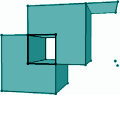
\includegraphics[width=12.0cm]{figs/teaser}}
%%     \caption{Demo application running on Windows. A polygon mesh is 
%%              subdivided using the quad-triangle subdivision 
%%              scheme~\cite{sl-qts-02}.}
%%     \label{fig:teaser}
%% \end{figure}



%% % open

%% Open source and contributions are welcome. 


%% % remainder

%% Section 2 describes how to declare a polyhedron, read a polygon mesh
%% from a file, and iterate over all facets for rendering. Example is
%% shown to enrich a polyhedron with extended primitives (normals,
%% colors, curvature tensors).

%% Section 3 illustrates how to write subdivision algorithms for meshes
%% (since they act on both connectivity and geometry, it is perfect for
%% our training purpose). Three approaches are shown. First one is sqrt3
%% subdivision using Euler operators. Second one uses the incremental
%% builder (originally designed for file IO) with a control mesh as
%% input. Third one offers a generic design for writing subdivision
%% algorithms.



%% % Andy

%% %program 1: rendering and file io of a default polyhedron 
%% %   context: a skeleton of a polyhedron program: declaration,
%% %initialization (inc. builder) and the rendering (iteration on facet and
%% %circulation of the factes)

%% %program 2: enriched polyhedron in program 1
%% %   context: extend a polyhedron: trait, item. hds? Use of the extended
%% %primitives.

%% %program 3: subdivision 1 (sqrt3)
%% %   context: refinement operators. Halfedge trversal (prev(), etc...) and
%% %circulators. Effect of connectivity edit on iterator and circulator.
%% %Maintain the correspondence after refinement.

%% %program 4: subdivision 2 (qt)
%% %   context: inc builder revisited.

%% %program 5: subdivisions (templated rules)
%% %   context: a generic design of subdivisions.

%% %program 2 is based on program 1 and program 3, 4, 5 are separate library
%% %functions called by program 2.

%% %The tutorial will walk though the programs. And a possible structure is
%% %sect 1: intro
%% %sect 2: program 1 & 2
%% %sect 3: program 3 & 4 & 5
%% %sect 4: conclusion 
        







